\documentclass[11pt]{article}

%\usepackage[english]{babel}
\usepackage[utf8]{inputenc} %German Umlaute :-)
\usepackage{apacite} %won't work for Greg, will work for Eva
%\usepackage{natbib} %will work for Greg, won't work for Eva
\usepackage{amsmath,amssymb}
\usepackage{graphicx}
\usepackage{color}
\usepackage{url}
\usepackage{fullpage}
\usepackage{setspace}
\usepackage{booktabs}
%\usepackage{lingmacros}
\usepackage{gb4e}
\usepackage{hyperref}
\hypersetup{colorlinks,breaklinks,
            linkcolor=cyan,urlcolor=cyan,
            anchorcolor=cyan,citecolor=cyan}


% useful commands
\definecolor{Red}{RGB}{255,0,0}
\newcommand{\red}[1]{\textcolor{Red}{#1}}
\newcommand{\jd}[1]{\textcolor{Red}{[jd: #1]}} 

\newcommand{\denote}[1]{\mbox{ $[\![ #1 ]\!]$}}
\newcommand{\subsubsubsection}[1]{{\em #1}}
\newcommand{\eref}[1]{(\ref{#1})}
\newcommand{\tableref}[1]{Table \ref{#1}}
\newcommand{\figref}[1]{Figure \ref{#1}}
\newcommand{\appref}[1]{Appendix \ref{#1}}
\newcommand{\sectionref}[1]{Section \ref{#1}}


%for margin notes
\usepackage{marginnote, setspace}
\newcommand{\evanote}[1]{%
   \marginnote{%
      \begin{spacing}{1}
         \vspace{-\baselineskip}%
         \color{OliveGreen}\footnotesize\singlespacing\itshape#1
      \end{spacing}
   }
}

\newcommand{\gcs}[1]{\textcolor{blue}{[gcs: #1]}} 


\title{The weakness of epistemic \emph{must}: Experimental evidence for a pragmatic reasoning approach}
 
\author{{\large \bf Judith Degen (jdegen@stanford.edu)}, \\ {\large \bf Gregory Scontras (scontras@stanford.edu),}\\ {\large \bf Andreas Trotzke (andreas.trotzke@uni-konstanz.de),}\\ {\large \bf Eva Wittenberg (ewittenberg@ucsd.edu)}}



\begin{document}

\maketitle

\begin{abstract}

We present a series of experiments suggesting that the epistemic necessity modal \emph{must} receives its notoriously weak interpretation by non-truth-conditional means of pragmatic reasoning, rather than by its lexical semantics. Specifically, we investigate the extent to which the interpretation of epistemic \emph{must} differs in strength from the interpretation of weaker modals and statements with no modals at all. We then propose a pragmatic account of the differences. To substantiate our claim that the interpretation of epistemic \emph{must} is not part of the descriptive part of the utterance, we also tested German discourse particles, showing that the German counterpart of \emph{must} patterns with these non-propositional means of expressing that the speaker commitment to the proposition is weakened.	
\end{abstract}

\textbf{Keywords:} 
pragmatics; semantics; psycholinguistics; modals; discourse particles; German; English


\section{Introduction}

When speakers are sure about some fact \emph{p}, they are likely to communicate this fact with a simple declarative utterance, as in (\ref{bare}). When they want to convey epistemic uncertainty, they have different possibilities: adding a modal adverbial, such as \emph{probably} (\ref{prob}), or using a modal verb, such as \emph{might} (\ref{might}). Either option leaves open the possibility that \emph{p} is not true.

\begin{exe}
	\ex\label{english} \begin{xlist}
		\ex\label{bare} The coffee is cold.
		\ex\label{prob} The coffee is probably cold.
		\ex\label{might} The coffee might be cold.
		\ex\label{must} The coffee must be cold.
	\end{xlist}
\end{exe}


Epistemic \emph{must} has a similar effect: (\ref{must}) communicates epistemic uncertainty, resulting in a weaker claim than the simple bare utterance in (\ref{bare}) \citep{karttunen1972}. The relative weakness of \emph{must} is puzzling because \emph{must} serves as a strong modal of necessity. Under a quantificational treatment of modality, these necessity modals correspond to universal quantifiers over possible worlds (XXX citation). They assert that in every (relevant) possible world, the proposition \emph{p} holds. So in (\ref{must}), epistemic \emph{must} should assert that in every world compatible with the speaker's knowledge, the coffee is cold. Given that knowledge corresponds to justified true belief (i.e., that which is known cannot be otherwise), from (\ref{must}) it necessarily follows that the coffee is cold (i.e., it is not possible that the coffee is not cold). There are other analyses of modals on the market (e.g., a scalar semantics for modals; \citealp{lassiter2011}), but all of them share the intuitive understanding of necessity modals as maximally strong semantic objects.

At issue, then, is the failed inference from (\ref{must}) to (\ref{bare}): How could \emph{must p} not entail \emph{p}? If the coffee is necessarily cold, then surely it is cold. It appears that talking about what is \emph{necessarily} the case commits speakers to less than does talking about what is \emph{actually} the case. \cite{karttunen1972} claimed that the inference from (\ref{must}) to (\ref{bare}) fails because \emph{must p} is a logically weaker statement than bare \emph{p}. In other words, the weakness of \emph{must} gets engineered into its lexical semantics. 

Thus, the original ``\emph{must} is weak'' mantra, stemming from \cite{karttunen1972}, has \emph{must p} not entail \emph{p}. There are two tacks to breaking this entailment. For \cite{kratzer1991}, the entailment fails because  \emph{must p} is weaker than we might have thought. She weakens \emph{must} by having it quantify not just over knowledge states, but also over expectations given knowledge states -- expectations which are not always borne out. For \cite{veltman1985}, the entailment fails because bare \emph{p} is stronger than we might have thought. He strengthens bare \emph{p} by allowing partial knowledge states, such that \emph{must p} may be true while we lack the knowledge to say whether \emph{p} is true or false. Either way, from \emph{must p} (e.g., ``It must be raining'') it does not follow that \emph{p} (e.g., ``It is raining'').

\cite{vonfintelgillies2010} present an alternative approach, arguing that \emph{must p} is indeed strong, quantifying universally over epistemically possible worlds. To account for the weak epistemic reading, they claim that \emph{must} is an evidential marker, presupposing that the speaker has no direct evidence of \emph{p}. However, the strength of \emph{must p} requires the speaker to have direct evidence of something that entails \emph{p}. Using a corpus of naturally-occurring examples from Ancestry.com, \citeauthor{lassiter2014salt} (\emph{to appear}) shows how \citeauthor{vonfintelgillies2010}'s implementation of a strong semantics for \emph{must} makes unreasonable claims about the knowledge states of speakers. \citeauthor{lassiter2014salt} proposes instead a weak probabilistic semantics: \emph{must p} entails that the probability of \emph{p} given the speaker's direct knowledge is greater than chance, and requires that the question of \emph{whether} \emph{p} not be resolved by this direct knowledge. Thus, \citeauthor{lassiter2014salt} returns to the original mantra of weakness while building evidential information into the semantics of \emph{must}.

Other languages have many more ways to convey epistemic uncertainty (for an overview, see \textbf{Drubig2001,Nuyts2001}). Some of these languages, like German, also offer non-propositional means for expressing weakened commitment, like discourse particles (e.g. \textbf{Zimmermann, 2011}). German is an interesting comparison case to English, since its other devices of expressing speaker commitment do not differ from English: Examples \ref{bareG}-\ref{mustG} are the German equivalents to \ref{bare}, \ref{prob}, and \ref{must}, while (\ref{wohlG}) is an example involving the discourse particle \emph{wohl} (\textbf{Zimmermann 2004}).

\begin{exe}
	\ex\label{german} \begin{xlist}
		\ex\label{bareG} Der Kaffee ist kalt geworden.
		\ex\label{probG} Der Kaffee ist vermutlich kalt geworden.
		\ex\label{mustG} Der Kaffee muss kalt geworden sein. 
		\ex\label{wohlG} Der Kaffee ist wohl kalt geworden.
	\end{xlist}
\end{exe}

What is interesting about (\ref{wohlG}) in our context is that discourse particles such as \emph{wohl} are not part of the propositional, truth-conditional content of an utterance, in contrast to modal adverbs such as \emph{vermutlich} (‘presumably’). For \emph{wohl}, Zimmermann (2004, 2008) has shown that this particular particle cannot affect the presuppositional domain of utterance interpretation, unlike modal adverbs such as \emph{vermutlich}. Specifically, if \emph{wohl} would semantically contribute to the proposition, its use in the following case should have the effect that the presupposition is an assumption rather than an actual state of affairs (capitals indicate focal stress):\\\textbf{
(let's do formatting after content -- SP squibs has its own formatting thing for glosses I think)}\\
(3)	a.	Peter	ist	\{ \#	wohl  	vermutlich\}	GESTERN	\\
		Peter	is		PRT     presumably	yesterday\\
			
		
		nach	 Hamburg	 gefahren,	\\
		to	 Hamburg	 driven	\\		
	b.	… vielleicht fährt er		\\
		aber	auch erst MORGEN.\\
		‘but maybe he will only go 
		tomorrow.’
	
	
	
As we see in (3), only the modal adverb \emph{vermutlich} can be mapped onto the background of a structured proposition, since only the modal adverb, and not the discourse particle, is felicitous given the continuation (3b), expressing an assertion that is in conflict with the presupposition of the utterance without \emph{wohl} or \emph{vermutlich}. Based on such evidence, many people have argued that discourse particles like \emph{wohl}, although in principle synonymous with certain adverbs (here: \emph{vermutlich}), operate within a separate, `use-conditional' meaning dimension (cf. Gutzmann 2015: 215-268 for more arguments).}
	
Coming back to epistemic must in English, in this paper we provide evidence that the weakness of epistemic \emph{must} need not derive from truth-conditional content (e.g., quantification over a limited set of possible worlds or presuppositions about evidence strength). First, we investigate what gets communicated via the use of \emph{must}. Over the course of three experiments, we asses the speaker commitments, evidence strength, and listener understanding that accompany \emph{must} statements, comparing \emph{must} to other modals and to statements with no modal at all. Our findings qualitatively confirm \citeauthor{karttunen1972}'s original observation, and quantitatively demonstrate the relative weakness of \emph{must}. Moreover, they highlight the role of evidence strength in the computation of \emph{must}'s meaning.

We then use our findings to motivate a pragmatic account of the relative weakness of \emph{must}. Rather than engineering weakness relative to bare \emph{p} directly into the meaning of the word, our account derives its weakness as an M-implicature \cite{grice1989,levinson2000}: \emph{must p} is marked (i.e., costly) relative to the bare form (\ref{bare}); the bare form is sufficiently strong already to convey \emph{p} (e.g., that it is raining), so listeners take the marked form to convey the marked meaning that the speaker arrived at the conclusion \emph{p} via an evidentially less certain route than if they had chosen the shorter, bare form. Our account obviates the conceptual pitfalls of \citeauthor{vonfintelgillies2010}'s strong semantics, without treating \emph{must} as inherently weak: evidence strength is inferred from, rather than communicated by, the use of \emph{must}. 

In order to further substantiate our claim, we consider \emph{must} from a cross-linguistic perspective, comparing \emph{must} to use-conditional means of expressing weakened speaker commitment that are not available in English. We therefore conducted the same series of experiments using German instead of English data. In particular, our experimental evidence suggests that speakers are more committed to a proposition \emph{p}/have stronger evidence for \emph{p} when they use German discourse particles instead of synonymous adverbs. As we have shown above, discourse particles expressing weakening commitment do not encode this weakening at the level of truth-conditional semantics, but rather at a separate use-conditional level. As \textbf{(3) }has shown, in the case of particles expressing (epistemic) uncertainty, this has the effect that the presupposition of an utterance is not an assumption (an expression of uncertainty). In other words, in terms of presuppositional semantics, the particle leaves the asserted state of affairs untouched, and thus we expect the speaker to be more committed to the truth of the proposition when using a particle than when using a synonymous adverb expressing weakened commitment. Since epistemic \emph{must} (German \emph{muss}) displays similar commitment patterns, we argue that the lexical/conventional meaning of \emph{must} stays strong and distinguishes \emph{must} from other modal means such as adverbs or verbs like \emph{might}. Accordingly, we consider our evidence as supporting our pragmatic account: the relatively weak interpretation of \emph{must} does not require encoding weakness or indirectness into the semantics of modals. When the cost of uttering \emph{must p} is greater than the bare form, a pragmatic listener jointly infers that $p(q)$ is smaller than when the utterance is the less costly bare $q$ and that the speaker has weak or imperfect evidence of $q$; the semantics of \emph{must} remains strong, but pragmatics does the job of weakening it.

%In sum, we take the following series of experiments to show that, at the conceptual level, our approach incorporates elements from both von Fintel and Gillies () and Lassiter to appear: \emph{Must} is lexically strong, and only pragmatic reasoning about its strong meaning yields a weaker interpretation. More specifically, we propose that the interpretation of epistemic \emph{must} is derived as an M-implicature (Grice, 1989; Levinson, 2000): must p (1c, 2c) is marked relative to the bare form (1a, 2a); the bare form conveys already that the coffee is cold (p), so listeners take the marked form to convey the marked meaning that the speaker arrived at the conclusion p via an evidentially less certain route than if they had chosen the unmarked bare form.


%Our first task is to evaluate the relative strength of \emph{must}, an empirical investigation conspicuously absent from the discussion of this modal thus far. Having justified the strength of \emph{must} empirically, we may then set our sights on the proposals meant to account for \emph{must}'s meaning.
 

%Abstract October
%Since Karttunen (1972), semanticists have debated how to account for the relatively weak mean-ing of epistemic must (1b) compared to bare utterances without a modal (1a). Rather than engi-neering the weakness of must into the lexical semantics (Lassiter, 2014), and rather than , 
%We further argue that epistemic must patterns cross-linguistically with non-propositional means of expressing weakened commitment towards the truth of the proposition: In English, speaker uncertainty is usually expressed by modal verbs (‘might’) or adverbs (‘probably’), both of which enter directly into the semantic calculation of a proposition. 
%To assess evidence strength, speaker commitments, and listener understanding in propositions employing must, propositional, and non-propositional epistemic means, we conducted two groups of studies in English and German.
% OLD INTRO:

%Modals come in varying degrees of strength; the 
%

%
%%
%Linguists split on the semantics of \emph{must}. 
%
%%
%In an effort to inform this debate on the strength of \emph{must}, we first investigate what gets communicated via its use. Over the course of three experiments, we asses the speaker commitments, evidence strength, and listener understanding that accompany \emph{must} statements. Our findings qualitatively confirm \citeauthor{karttunen1972}'s original observation, and quantitatively demonstrate the relative weakness of \emph{must}. Moreover, they highlight the role of evidence strength in the computation of \emph{must}'s meaning -- an ingredient that has thus far been lacking from the proposed semantics for \emph{must}.
%
%We then use our findings to motivate a computational model of the meaning of \emph{must}, following \citeA{lassitergoodman2013} in their extension of the Bayesian Rational Speech Act framework \cite{frankgoodman2012}. Rather than engineering weakness relative to bare \emph{p} directly into the meaning of the word \emph{must}, our account derives its weakness as an M-implicature \cite{levinson2000}: \emph{must p} is marked (i.e., costly) relative to the bare form (\ref{bare}); the bare form is sufficiently strong already to convey \emph{p} (e.g., that it is raining), so listeners take the marked form to convey the marked meaning that the speaker arrived at the conclusion \emph{p} via an evidentially less certain route than if they had chosen the shorter, bare form. Our account accomplishes two things. First, it obviates the conceptual pitfalls of \citeauthor{vonfintelgillies2010}'s strong semantics, without treating \emph{must} as inherently weak: evidence strength is inferred from, rather than communicated by, the use of \emph{must}. Second, it implements a formal model of M-implicatures within the Rational Speech Act framework \cite{bergenetal2014}.
%
%Our approach incorporates elements from both \citeA{vonfintelgillies2010} and \citeauthor{lassiter2014salt} \emph{to appear}: \emph{Must} is strong, but reasoning about its strong meaning yields a weaker interpretation.

\section{Experiment 1: evidence strength}

In Exp.~1, we collected estimates of evidence strength.\footnote{The English version of this experiment can be viewed \href{https://web.stanford.edu/~justinek/modals_exp/evidence.html}{here}. The German version can be viewed \href{http://web.stanford.edu/~jdegen/cgi-bin/4_dp_priors_evidencestrength/evidence.html}{here}.} These estimates were used in the analysis of Experiments 2 and 3.

\subsection{Methods}

\subsubsection{Participants}

For the English version, 40 native English speakers were recruited through Amazon's Mechanical Turk crowd-sourcing service. For the German version, 40 German native speakers were recruited through Clickworker's crowd-sourcing service. Both groups were compensated for their participation.

\subsubsection{Materials and procedure}

Participants rated the probability of a state of affairs $q$ given a piece of evidence $e$ by adjusting a slider on a scale with endpoints labeled ``impossible'' and ``absolutely certain''. On each trial, participants first saw the context sentence ``Imagine that you are at home.'' Then the evidence $e$ for $q$ was shown, e.g., ``Dinner is usually ready around 6pm. You look at the clock and it is 6pm.'' Finally, participants were asked about the probability of $q$, e.g., ``How likely is it that dinner is ready?'' and adjusted the slider accordingly. There were four different $q$ that appeared in the ``How likely is it that $q$?'' frame:

\begin{exe}
	\ex it is raining
	\ex the coffee is cold
	\ex dinner is ready
	\ex the neighbor's dog is barking
\end{exe}

For each \emph{q}, each participant evaluated one of five possible pieces of evidence, resulting in four trials per participant. Trial order was randomized. 

Pieces of evidence were generated by taking a version of the top five most frequently generated explanations from a separate experiment in which $q$ was given to participants and they were asked to provide a free response explanation of how the speaker knows about $q$.\footnote{This experiment can be viewed \href{http://stanford.edu/~jdegen/68_modals_freeproduction/modals.html}{here}.} The full list of pieces of evidence for each $q$ can be found in \appref{sec:evidence}.

For the German version, the procedure was identical; all materials were translated into German. See \appref{sec:evidence} for the full list of stimuli.

\subsection{Results and discussion}

\subsubsection{English.}
We obtained between 3 and 14 ratings for each piece of evidence. We interpret the slider value between 0 (``impossible'') and 1 (``absolutely certain'') as a participant's estimate of the probability of $q$, given $e$, which we will also sometimes refer to as  \emph{evidence strength}. A histogram of mean evidence strengths is shown in \figref{fig:evidencestrength}.  We used these evidence strength ratings in the design and analyses of Experiments 2 and 3.

\begin{figure}
\centering
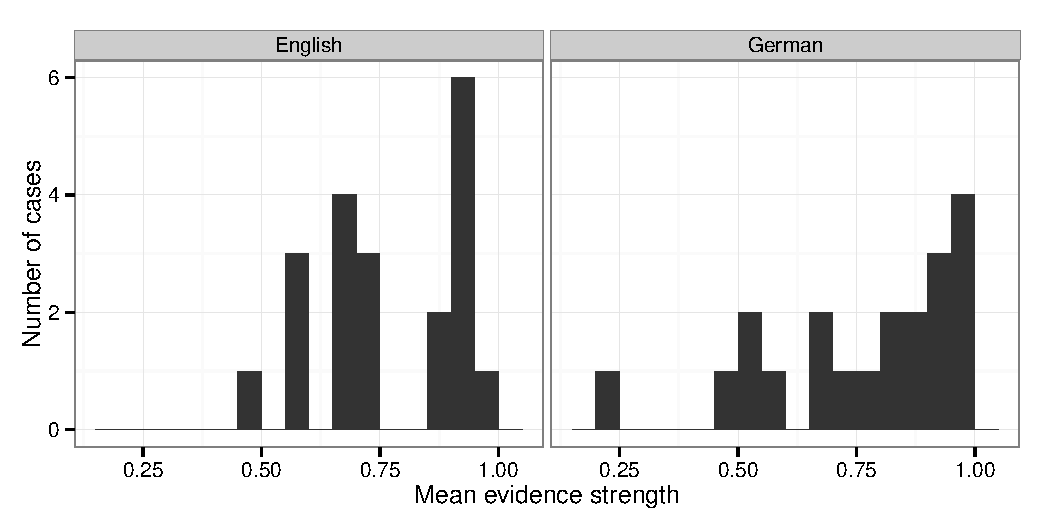
\includegraphics[width=.9\textwidth]{pics/evidencestrength-histograms}
\caption{Histogram of by-item evidence strength means  for English (left) and German (right).}
\label{fig:evidencestrength}
\end{figure}

%\begin{figure}
%\centering
%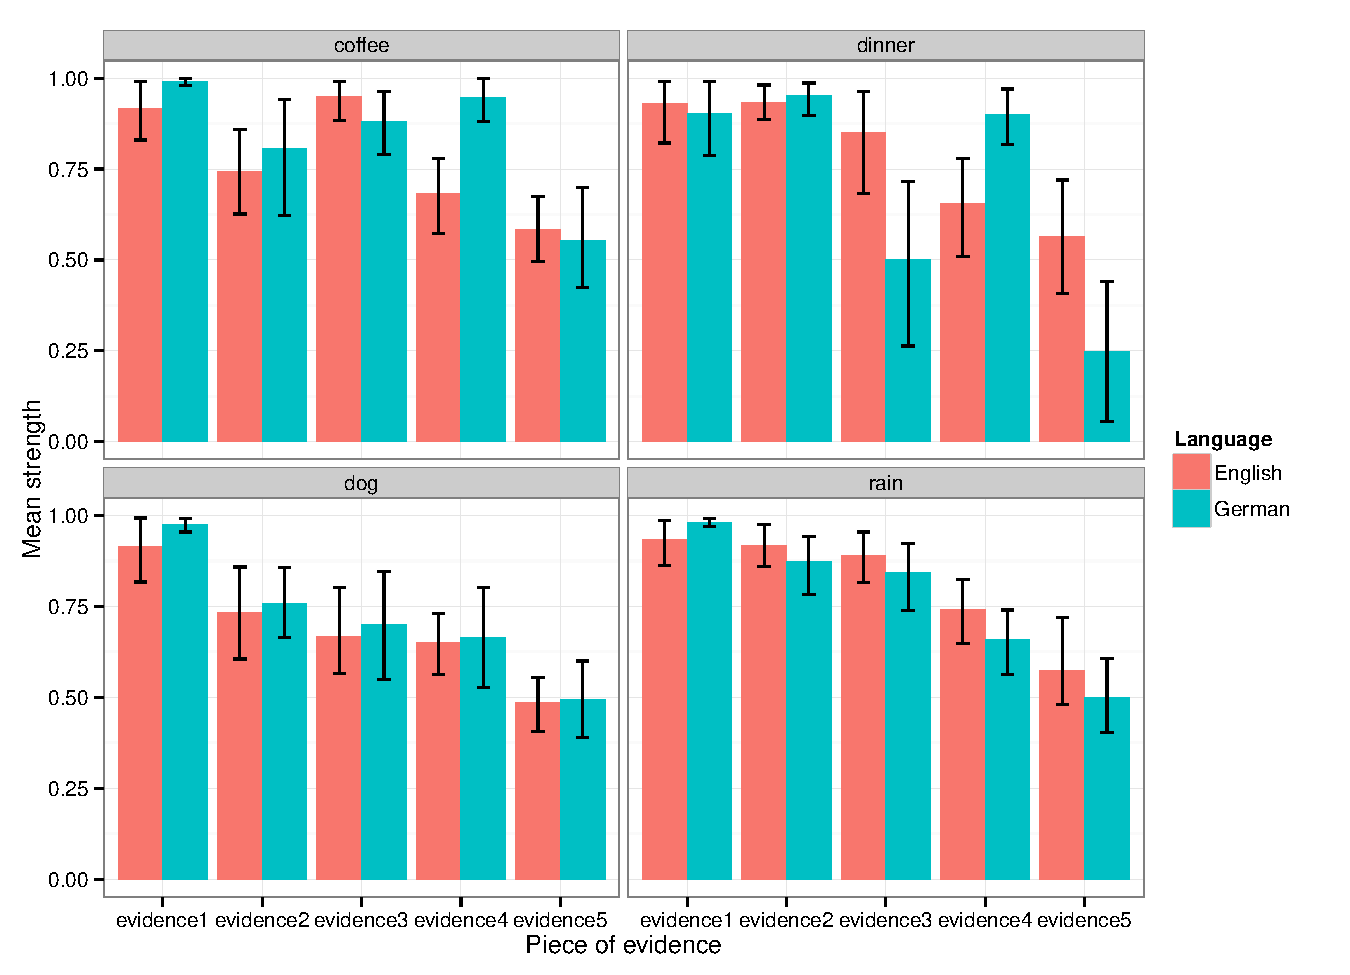
\includegraphics[width=\textwidth]{pics/mean-evidencestrength-byitem}
%\caption{Mean by-item evidence strength for English and German, by domain. Error bars are bootstrapped 95\% confidence intervals.\red{THIS IS MOSTLY JUST FOR YOU GUYS TO HAVE A LOOK, unless you think this sort of plot would be useful to include. Basically, there are }}
%\label{fig:evidencestrength}
%\end{figure}

\subsubsection{German.}
We obtained between 3 and 14 ratings for each piece of evidence. Participants' estimates of evidence strength are shown alongside those of the English-speaking participants in  \figref{fig:evidencestrength}. To test whether the English and German distributions of strength ratings differed, we conducted a mixed-effects linear regression predicting evidence strength rating from a dummy-coded fixed effect of language (with English as reference level) as well as by-participant and by-item random intercepts and by-item random slopes for language. The effect of language did not reach significance ($\beta$ = -.01, $SE$ = .03, $t$ = -.22, $p <$ .83), suggesting that the two populations did not differ in their estimates of evidence strength.   

\section{Experiment 2: production}

Next, we evaluated speakers' intuitions in a forced production task, testing how likely they are to use a particular form to communicate their belief about $q$ when given different pieces of evidence.\footnote{The English version of this experiment can be viewed \href{http://stanford.edu/~jdegen/71_modals_forced_production/modals.html}{here}.} The German version was identical with the exception that it was conducted in German and contained slightly different utterance choices.\footnote{The German version of this experiment can be viewed \href{http://web.stanford.edu/~jdegen/cgi-bin/3_dp_production/modals.html}{here}.}

\subsection{Methods}

\subsubsection{Participants}

For the English version, we recruited 40 participants from Amazon's Mechanical Turk. For the German version, we recruited 40 participants on the German crowd-sourcing service Clickworker. Participants were compensated with a small payment.

\subsubsection{Materials and procedure}

Participants were presented with a piece of evidence (e.g., ``You see a person come in from outside with wet hair and wet clothes'') and were asked to choose one of four possible utterances to describe the situation to a friend. On each trial, they first saw a context sentence which varied by domain, e.g., ``Imagine that you are sitting in a room.'' Next, they were presented with a piece of evidence, e.g., ``Earlier today, you had seen dark clouds in the sky.'' Finally, each participant saw the same question: ``Given what you know, what do you say to a friend who is sitting in a windowless room down the hall?'' They then chose one of four possible utterances by checking a radio button, e.g., ``It's raining'', ``It must be raining'', ``It's probably raining'', ``It might be raining''. Across domains, each choice was between utterances of the forms shown in \eref{utterancechoices}.

\begin{exe}
	\ex\label{utterancechoices} \emph{Abstract form of utterance choices:}
	\begin{xlist}
		\ex $q$ (bare)
		\ex \emph{must q} (must)
		\ex \emph{probably q} (probably)
		\ex \emph{might q} (might)
		\end{xlist}
		\end{exe}
		
Each participant completed 12 trials, three per domain. For each participant and domain, three pieces of evidence were randomly sampled from the set of five. Trial order was randomized, as was the order of utterance options.

The procedure for German was identical. As for participants' utterance choices, we included bare $q$ form and \emph{must q} as in the English version, but instead of the modals \emph{probably} and \emph{might}, we included the modal adverbial \emph{vermutlich} (English \emph{presumably}) and the discourse particle \emph{wohl}.

\subsection{Results and discussion}

\subsubsection{English.} The overall distribution of utterance choices is shown in \figref{fig:utterances}. The bare and \emph{might} forms are used most frequently, with both \emph{must} and \emph{probably} being chosen at only half the rate. The main question of interest in production, in contrast, is whether the choice of form to communicate about $q$ depends on the strength of the evidence for $q$. Indeed it does: \figref{fig:utterances-estrength} shows the mean strength of the evidence (as elicited in Exp.~E.1) that participants were given as a function of the utterance they ultimately chose.   In order to evaluate the effect of evidence strength on utterance choice, we conducted a mixed-effects linear regression predicting evidence strength from a dummy-coded predictor for utterance choice (with \emph{must} as reference level) as well as random by-participant and by-item  intercepts. Evidence strength was greater when the bare form was produced than when \emph{must q} was produced ($\beta$ = .11, $SE$ = .01, $t$ = 7.58, $p <$ .0001) and smaller when \emph{might q} was produced  ($\beta$ = -.13, $SE$ = .01, $t$ = -8.99, $p <$ .0001). There was no difference in evidence strength between \emph{must q} and \emph{probably q}  ($\beta$ = -.01, $SE$ = .02, $t$ = -.73, $p <$ .47). 

\begin{figure}
\centering
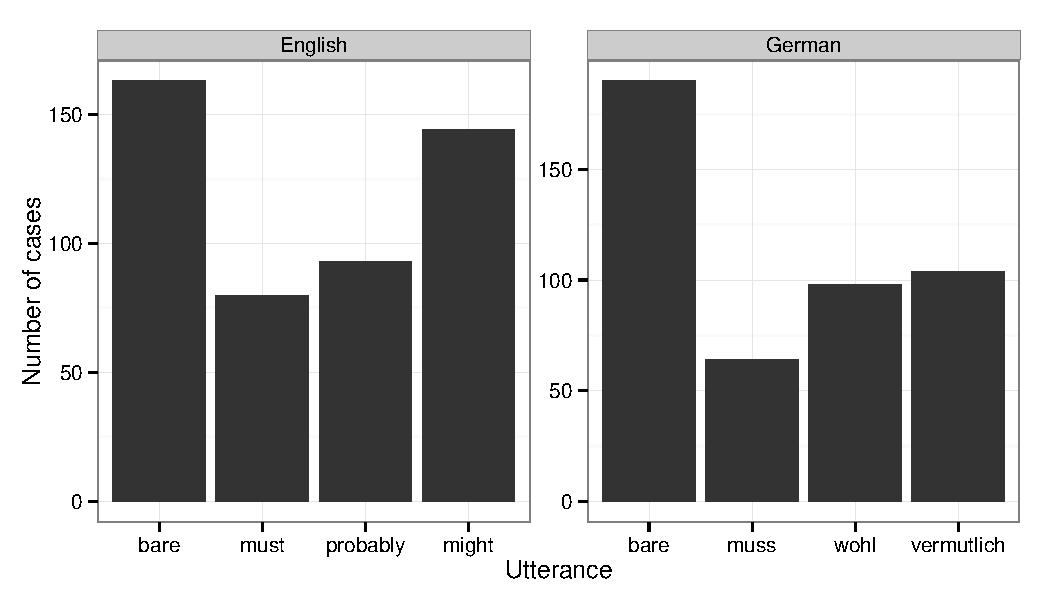
\includegraphics[width=.9\textwidth]{pics/production-distribution}
\caption{Histogram of utterance choice for English (left) and German (right).}
\label{fig:utterances}
\end{figure}

\begin{figure}
\centering
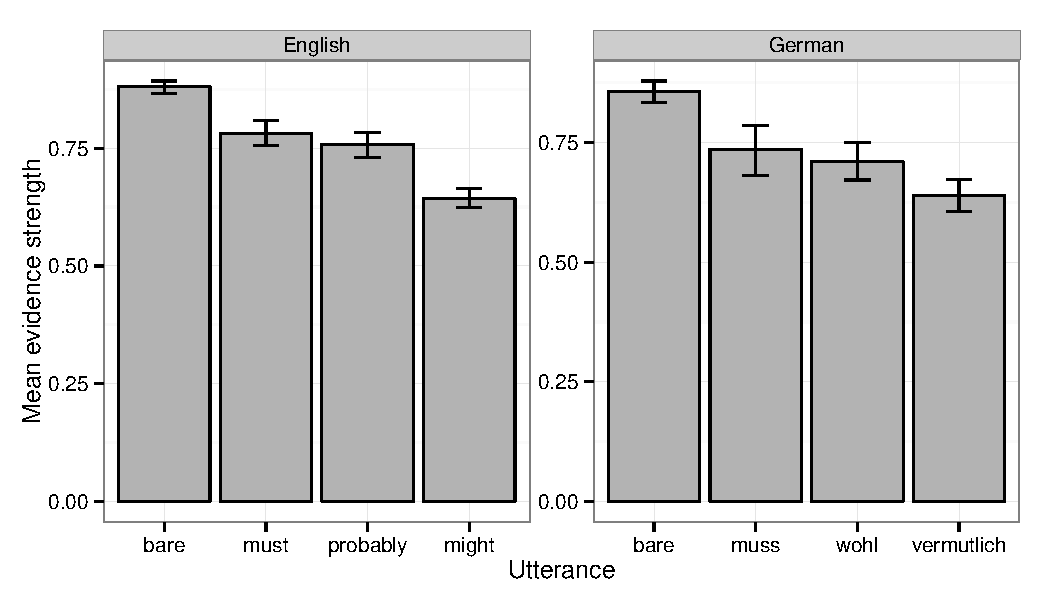
\includegraphics[width=.9\textwidth]{pics/mean-production-evidence}
\caption{Mean strength of evidence given when using each utterance, for English (left) and German (right). Error bars indicate bootstrapped 95\% confidence intervals.}
\label{fig:utterances-estrength}
\end{figure}


\subsubsection{German.} The overall distribution of utterance choices is shown in \figref{fig:utterances} alongside the English results. The bare form is used most frequently, with the other forms only being chosen half as often, and indeed, \emph{muss q} is dispreferred in general. We are again interested in whether the choice of form to communicate about $q$ depends on the strength of the evidence for $q$: mean strength of the evidence (as elicited in Exp.~E.1) that participants were given as a function of the utterance they ultimately chose is visualized in\figref{fig:utterances-estrength}.  Mirroring the English results, evidence strength was greater when the bare form was produced than when \emph{muss q} was produced ($\beta$ = .12, $SE$ = .03, $t$ = 4.78, $p <$ .0001). In addition, evidence strength was smaller when \emph{vermutlich q} was produced  ($\beta$ = -.09, $SE$ = .03, $t$ = -3.35, $p <$ .0009). Crucially, there was no difference in evidence strength between \emph{muss q} and \emph{wohl q}  ($\beta$ = -.02, $SE$ = .03, $t$ = -.67, $p <$ .51). 

\subsection{Discussion}
We interpret these results as follows. In German, due to the lexical inventory of discourse particles, speakers have a choice of using epistemic adverbs such as \emph{vermutlich}, epistemic \emph{muss}, and particles like \emph{wohl}. As Figure 4 shows, speakers tend to use \emph{muss} and \emph{wohl} instead of the respective adverb when the degree of evidence strength is higher. In other words, when investigating the dependence on evidence strength for q, we find that \emph{muss} and \emph{wohl} pattern, in contrast to other modal means such as \emph{vermutlich}. This is in line with the fact introduced in Section 1 above that discourse particles, in contrast to modal adverbs, do not add epistemic uncertainty to the presupposition of an utterance. As we want to argue in this paper, epistemic must also does not add the effect of weakened commitment to the presupposition of an utterance. Rather, this effect is derived by pragmatic reasoning.

\section{Experiment 3a: comprehension (listener belief)}

%Having found that speakers' use of \emph{must} increases as evidence strength decreases, we next tested whether listeners take into account this information about speakers as they interpret the bare and \emph{must} forms. In testing listeners' interpretation of \emph{must}, we also evaluated its relative strength.

We next tested the other side of the communicative coin: depending on the utterance $u$ used to communicate about $q$, how strong is listeners' resulting belief in $q$, and what do they believe to be the strength of the evidence the speaker was in possession of when producing $u$?\footnote{The English version of this experiment can be viewed \href{http://stanford.edu/~jdegen/72_modals_comprehension_evidence_room/modals.html}{here}.} The German experiment was identical, with the exception that it was conducted in German and included the slightly different set of utterance options used in the German version of Experiment 2. \footnote{The German version of this experiment can be viewed \href{http://web.stanford.edu/~jdegen/cgi-bin/2_dp_comprehension_listenerbelief/modals.html}{here}.}

\subsection{Methods}

\subsubsection{Participants}

For the English version, we recruited 60 participants through Amazon's Mechanical Turk. 
For the German version, we recruited 60 participants through the German crowd-sourcing service Clickworker. Participants were compensated with a small payment.

\subsubsection{Materials and procedure}

Participants were presented with an utterance (e.g., ``It must be raining'') and asked a) to rate the probability of the state of affairs \emph{q} (e.g., it is raining); and b) to select one out of five pieces of evidence that the speaker had about \emph{q} in making their utterance. On each trial, participants first saw two context sentences: ``You are in a windowless room. Your friend X walks in and says:'', where ``X'' was a randomly generated name.\footnote{This was done to discourage effects of inferences about speaker-specific language use on interpretation.} Participants then saw one of the utterances from Exp.~E.2 that ``X'' produced, e.g., ``It must be raining''. They were asked ``How likely do you think it is that it is raining?'' and adjusted a slider with endpoints labeled ``impossible'' and ``certain'' in response. Once they thus submitted their belief in $q$, the five potential pieces of evidence previously used in Exps.~E.1 and E.2 were shown and participants were asked to choose one by clicking a radio button in response to the question ``How do you think X knows about the rain?'' 

Participants provided one set of judgments for each domain, resulting in four trials per participant. Each participant saw each type of utterance (bare, must, probably, might)  across trials. Utterance types were randomly distributed across domains. Trial order was randomized, as was the order in which pieces of evidence were displayed.

In the German version, the procedure was identical, but materials were presented in German and the utterances participants observed were the ones used in the German version of Experiment 2.

\subsection{Results and discussion}

\subsubsection{English.} Two questions are of interest: first, does the probability of listener belief in $q$ vary as a function of the observed utterance? Second, does the strength of the evidence for $q$ inferred to be available to the speaker vary as a function of the observed utterance? To address the first question, we conducted a mixed effects linear regression predicting degree of belief in $q$ from a dummy-coded utterance predictor with \emph{must} as reference level. The model included random by-participant and by-item intercepts. Fig.~\ref{fig:expt3} shows mean probability of listener belief in $q$ by utterance: participants believed \emph{q} was more likely after observing the bare utterance than after observing the \emph{must} utterance   ($\beta$=.24, \emph{SE}=0.03, \emph{t}=9.1, \emph{p}$<$0.0001). In contrast, they believed $q$ was less likely after observing \emph{might q} ($\beta$=-.09, \emph{SE}=0.03, \emph{t}=-3.44, \emph{p}$<$0.0008). There was no difference in resulting listener belief between \emph{must q} and \emph{probably q} ($\beta$=-.04, \emph{SE}=0.03, \emph{t}=-1.6, \emph{p}$<$0.12). These results mirror the evidence strength effects found in production (Exp.~E.2). 

To address whether inferred speaker evidence strength mirrors production, we conducted another mixed effects linear regression, predicting inferred strength of evidence for $q$ from a dummy-coded utterance predictor with \emph{must} as reference level. The model included random by-participant and by-item intercepts.  \figref{fig:exp3-evidence} shows mean evidence strength ascribed to speakers by utterance:  interestingly, participants inferred stronger evidence was available to the speaker after observing the bare utterance than \emph{must q} ($\beta$=.08, \emph{SE}=.02, \emph{t}=3.74, \emph{p}$<$ .0003), but inferred evidence strength was no different for \emph{probably q} ($\beta$=.01, \emph{SE}=0.02, \emph{t}=.55, \emph{p}$<$ .59) or \emph{might q} ($\beta$=-.02, \emph{SE}=0.02, \emph{t}=-.89, \emph{p}$<$ .38).

\begin{figure}
	\centering
	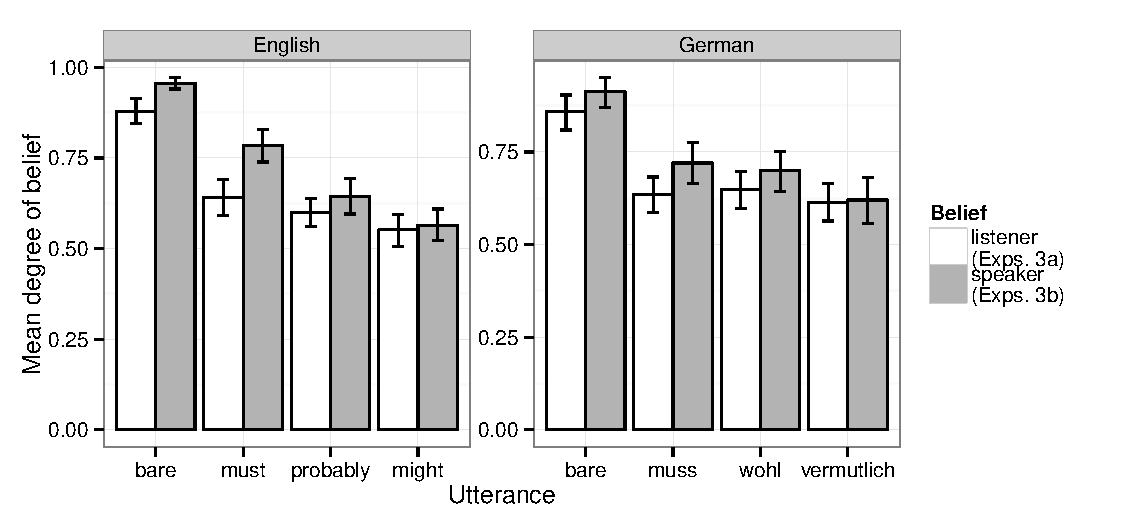
\includegraphics[width=\textwidth]{pics/mean-beliefs}
	\caption{Mean probability of listener and speaker belief in $q$ by utterance for English (left) and German (right). Error bars indicate 95\% bootstrapped confidence intervals.}
	\label{fig:expt3}
\end{figure}

\begin{figure}
	\centering
	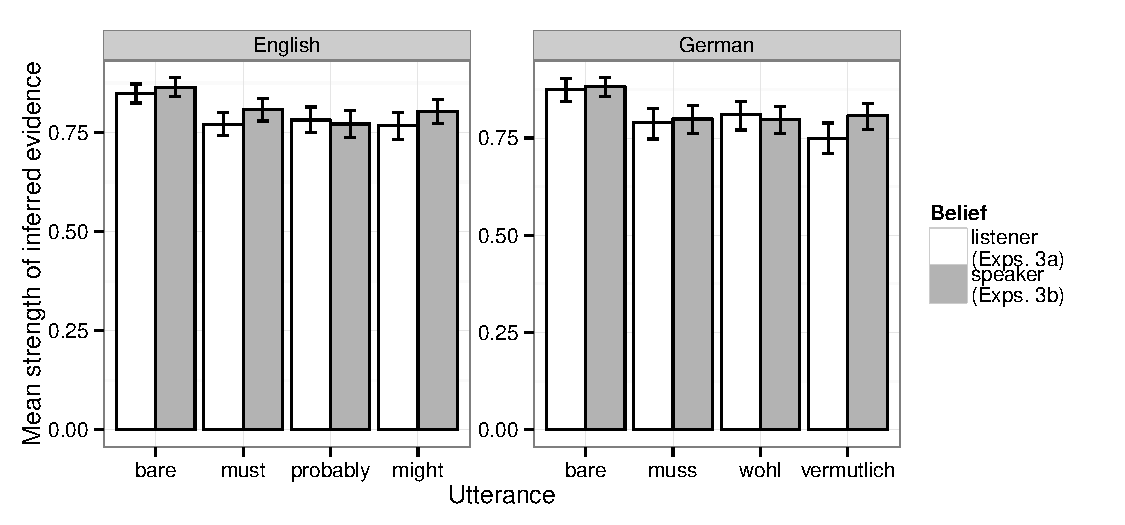
\includegraphics[width=\textwidth]{pics/mean-evidence}
	\caption{Mean inferred evidence strength by utterance for English (left) and German (right). Error bars indicate 95\% bootstrapped confidence intervals.}
	\label{fig:exp3-evidence}
\end{figure}

\subsubsection{German.} Fig.~\ref{fig:expt3} shows mean probability of listener belief in $q$ by utterance alongside the English results: participants believed \emph{q} was more likely after observing the bare utterance than after observing the \emph{muss} utterance   ($\beta$=.22, \emph{SE}=0.03, \emph{t}=7.5, \emph{p}$<$0.0001). However, there were no differences in degree of belief in $q$ between \emph{muss q} and \emph{vermutlich q} ($\beta$=-.02, \emph{SE}=0.03, \emph{t}=-.76, \emph{p}$<$.46) nor between \emph{muss q} and \emph{wohl q} ($\beta$=.01, \emph{SE}=0.03, \emph{t}=.43, \emph{p}$<$.67). 

Fig.~\figref{fig:exp3-evidence} shows mean evidence strength ascribed to speakers by utterance alongside the English results: as in the German case, participants inferred stronger evidence was available to the speaker after observing the bare utterance than \emph{muss q} ($\beta$=.08, \emph{SE}=.02, \emph{t}=3.23, \emph{p}$<$ .002). In addition, they inferred that the available evidence must have been weaker upon observing \emph{vermutlich q} ($\beta$=-.05, \emph{SE}=.02, \emph{t}=-2.1, \emph{p}$<$ .04), but inferred evidence strength was no different for \emph{wohl q} ($\beta$=.001, \emph{SE}=0.02, \emph{t}=.07, \emph{p}$<$ .95).

\section{Experiment 3b: comprehension (speaker commitment)}

%Having found that speakers' use of \emph{must} increases as evidence strength decreases, we next tested whether listeners take into account this information about speakers as they interpret the bare and \emph{must} forms. In testing listeners' interpretation of \emph{must}, we also evaluated its relative strength.

Exp.~3a tested listener beliefs in $q$ as a function of the observed utterance. A related, but potentially orthogonal dimension is the commitment that listeners ascribe to speakers as a basis for producing a particular utterance. For example, a particular utterance may lead the listener to infer that the speaker is highly committed to $q$, while nevertheless not instilling the same degree of belief in $q$ in the listener. In fact, epistemic \emph{must} has been claimed to function like this: vFG claim that maximal speaker commitment is necessary for the use of epistemic \emph{must}, just as in the use of the bare form; yet in comprehension the interpretation of \emph{must q} is weaker than that of bare $q$.  Exp.~E.3b thus tested the degree of belief in $q$ that listeners ascribe to \emph{speakers} depending on the utterance the speaker produced.\footnote{This experiment can be viewed \href{http://stanford.edu/~jdegen/80_modals_comprehension_speakerbelief/modals.html}{here}. The German version can be viewed \href{http://web.stanford.edu/~jdegen/cgi-bin/1_dp_comprehension_speakerbelief/discourse_particles.html}{here}.}

\subsection{Methods}

\subsubsection{Participants}

We recruited 60 English native speakers through Amazon's Mechanical Turk, and 60 German native speakers through Clickworker. Participants were compensated with a small payment.

\subsubsection{Materials and procedure}

The design, procedure, and materials were identical to those of Exp.~3a with the exception of the dependent measure: instead of asking participants how likely they thought that $q$, they instead answered the question ``Does X think that it's raining?'' by adjusting a slider on a scale with endpoints labeled ``Definitely not'' and ``Definitely''. 

\subsection{Results and discussion}

\subsubsection{English.} As in Exp.~3a, two questions are of interest: first, does the probability of  belief in $q$ -- this time, as ascribed to the speaker rather than as the result of the listener's interpretation --  vary as a function of the observed utterance? Second, does the strength of the evidence for $q$ inferred to be available to the speaker vary as a function of the observed utterance? To address the first question, we conducted a mixed effects linear regression predicting degree of belief in $q$ from a dummy-coded utterance predictor with \emph{must} as reference level. The model included random by-participant and by-item intercepts. Fig.~\ref{fig:expt3} shows mean probability of ascribed speaker belief in $q$ by utterance: participants believed the speaker was more likely to believe \emph{q}  after observing the bare utterance than after observing the \emph{must} utterance   ($\beta$=.18, \emph{SE}=0.03, \emph{t}=6.59, \emph{p}$<$0.0001). In contrast, they believed the speaker was less likely to believe $q$ if they produced \emph{probably q} ($\beta$=-.14, \emph{SE}=0.03, \emph{t}=-5.28, \emph{p}$<$0.0001) or \emph{might q} ($\beta$=-.22, \emph{SE}=0.03, \emph{t}=-8.36, \emph{p}$<$0.0001). 

These results mirror the effects found in Exp.~E.3a, with the exception that all utterances led to differences in ascribed speaker commitment. Interestingly, the strength of the belief that participants attributed to speakers was stronger than their own resulting belief. This was borne out statistically in a model that was applied to both the listener and speaker belief datasets. This model was identical to that just reported, but additionally allowed for a dummy-coded belief holder predictor (listener vs.~speaker)  to interact with utterance. There was a clear main effect of belief holder, such that the belief ascribed to speakers was stronger than that held by listener participants ($\beta$=.14, \emph{SE}=0.03, \emph{t}=4.7, \emph{p}$<$0.0001). 

As in Exp.~E.3a, to address whether inferred speaker evidence strength mirrors production, we conducted another mixed effects linear regression, predicting inferred strength of evidence for $q$ from a dummy-coded utterance predictor with \emph{must} as reference level. The model included random by-participant and by-item intercepts.  \figref{fig:exp3-evidence} shows mean evidence strength ascribed to speakers by utterance:  again, participants inferred stronger evidence was available to the speaker after observing the bare utterance than \emph{must q} ($\beta$=.06, \emph{SE}=.02, \emph{t}=3.2, \emph{p}$<$ .002), but inferred evidence strength was no different for \emph{probably q} ($\beta$=-.02, \emph{SE}=0.02, \emph{t}=-1.11, \emph{p}$<$ .27) or \emph{might q} ($\beta$=-.01, \emph{SE}=0.02, \emph{t}=-.49, \emph{p}$<$ .63).

Allowing this model to interact with a belief holder predictor and applying it to simultaneously to the Exp.~E.3a dataset yields no main effect of belief holder ($\beta$=.03, \emph{SE}=.02, \emph{t}=1.53, \emph{p}$<$ .13) -- this is unsurprising, given that this aspect of the dependent measure was identical across experiments.

\subsubsection{German.} Fig.~\ref{fig:expt3} shows mean probability of ascribed speaker belief in $q$ by utterance alongside the English results: participants believed the speaker was more likely to believe \emph{q}  after observing the bare utterance than after observing the \emph{muss} utterance  ($\beta$=.19, \emph{SE}=0.03, \emph{t}=5.79, \emph{p}$<$ .0001). In contrast, they believed the speaker was less likely to believe $q$ if they produced \emph{vermutlich q} ($\beta$=-.1, \emph{SE}=0.03, \emph{t}=-3.01, \emph{p}$<$0.004). There was no difference between \emph{muss q} and \emph{wohl q} ($\beta$=-.02, \emph{SE}=0.03, \emph{t}=-.61, \emph{p}$<$ .55).  This shows, similar to what we found in the domain of production, that speaker commitment in the case of both epistemic \emph{must} and discourse particles is stronger than in the case of using otherwise synonymous adverbs such as \emph{vermutlich}. This finding is in accordance with our treatment of epistemic \emph{must} as an phenomenon that rests on non-presuppositional components of utterance meaning

Conducting the analysis jointly on the listener (Exp.~3a) and speaker  (Exp.~3b) belief data and allowing a belief holder predictor to interact with the utterance predictor again yields a main effect of belief holder such that the belief ascribed to speakers is stronger than the resulting belief in participants ($\beta$=.08, \emph{SE}=0.04, \emph{t}=2.23, \emph{p}$<$ .03).

As for Exp.~3a, \figref{fig:exp3-evidence} shows mean evidence strength ascribed to speakers by utterance alongside the English results; the qualitative results were identical to those in the English case. Participants inferred stronger evidence was available to the speaker after observing the bare utterance than \emph{muss q} ($\beta$=.08, \emph{SE}=.02, \emph{t}=4.05, \emph{p}$<$ .0001). However, evidence strength was not inferred to be any different after observing \emph{vermutlich q} ($\beta$=-.0003, \emph{SE}=.02, \emph{t}=-.02, \emph{p}$<$ .99) or \emph{wohl q} ($\beta$=.008, \emph{SE}=0.02, \emph{t}=.36, \emph{p}$<$ .72).

Allowing a belief holder predictor to interact with the utterance predictor when applied to both the listener and the speaker dataset yielded no effect of belief holder ($\beta$=.0008, \emph{SE}=0.03, \emph{t}=.04, \emph{p}$<$ .97).

\section{General discussion}
In this short paper, we presented a series of experiments supporting the idea that the epistemic modal \emph{must} receives its weak interpretation by non-truth-conditional means of pragmatic reasoning, rather than by its lexical semantics. Specifically, we investigate the extent to which the interpretation of epistemic \emph{must} differs in strength from the interpretation of weaker modals and statements with no modals at all. To substantiate our claim that the interpretation of epistemic \emph{must} is not part of the presuppositional part of the utterance, we also tested German discourse particles, showing that the German counterpart of \emph{must} patterns with these non-propositional means of expressing that the speaker commitment to the proposition is weakened. Accordingly, our experiments lend support to an account of epistemic \emph{must} that refrains from engineering the effect of weakness into the descriptive content of the utterance and assumes that the notorious weakening effect is part of a non-propositional domain of utterance interpretation. We thus hope that our studies provide an empirical base for further research on the pragmatic side of epistemic \emph{must}.



%\section{Model}

%We propose a computational model of language understanding to show that the empirically verified, relatively weak interpretation of \textit{must} does not require encoding weakness or indirectness into the semantics of modals, but can  arise instead from pragmatic reasoning about its strength. In fact, already in \citeA[pp.~33--34]{grice1989} do we find inspiration for the calculation that leads to the relative weakness of \emph{must}:
%
%\begin{quotation}
%	``A wants to know whether \emph{p}, and B volunteers not only the information that \emph{p}, but information to the effect that it is certain that \emph{p}\ldots\ B's volubility may be undesigned, and if it is so regarded by A it may raise in A's mind a doubt as to whether B is as certain as he says he is\ldots\ But if it is thought of as designed, it would be an oblique way of conveying that it is to some degree controversial whether or not \emph{p}.''
%\end{quotation}
%
%\noindent Here, we formalize \citeauthor{grice1989}'s description of the computation. 
%
%Our model follows the basic structure of Rational Speech Act (RSA) models, which view language understanding as recursive reasoning between speaker and listener \cite{frankgoodman2012}.

\appendix

\section{Pieces of evidence}
\label{sec:evidence}

This section lists, for each proposition $q$, the five pieces of evidence that were used throughout all experiments.

\subsection{It's raining. / Es hat geregnet.}

\begin{enumerate}
	\item You look out the window and see raindrops falling from the sky. \\ Sie sehen aus dem Fenster und beobachten, wie Regentropfen vom Himmel fallen. 
	\item You hear the sound of water dripping on the roof. \\ Sie können hören, wie Wasser auf das Dach prasselt.
	\item You check the weather report on the Internet, which says it is raining. \\ Sie haben im Internet den Wetterbericht gelesen, in dem stand, dass es regnen würde. 
	\item You see a person come in from outside with wet hair and wet clothes. \\ Sie sehen, wie jemand mit nassen Haaren und durchnässten Kleidern von draußen hereinkommt.
	\item Earlier today, you had seen dark clouds in the sky. \\ Sie haben heute Vormittag dunkle Wolken am Himmel gesehen.
\end{enumerate}

\subsection{The coffee is cold. / Der Kaffee ist kalt geworden.}

\begin{enumerate} 
	\item You take a sip of the coffee and feel that it is cold. \\
	Sie trinken einen Schluck Kaffee und stellen fest, dass er kalt ist
	\item You touch the coffee cup and feel that it is cold.\\
	Sie berühren die Kaffeetasse und stellen fest, dass sie kalt ist.
	\item You see that there is no steam coming from the coffee.\\
	Sie sehen, dass aus dem Kaffee kein Dampf aufsteigt.
	\item You know that the coffee has been on the table for an hour.\\
	Sie wissen, dass der Kaffee seit einer Stunde auf dem Tisch steht.
	\item You see that the cup isn't insulated.\\
	Sie sehen, dass die Tasse nicht isoliert ist.
\end{enumerate}

\subsection{Dinner is ready. / Das Abendessen ist fertig geworden.}

\begin{enumerate}
	\item You just prepared dinner and set it out on the table.\\
	Sie haben gerade das Abendessen zubereitet und auf den Tisch gestellt
	\item Your spouse tells you that dinner is ready.\\
	Ihr/e Partner/in sagt, dass das Abendessen fertig ist.
	\item Dinner is usually ready at around 6pm. You look at the clock and it is 6pm.\\
	Sie wissen, dass das Abendessen normalerweise um 18 Uhr fertig ist. Ein Blick auf die Uhr zeigt, dass es gerade 18 Uhr ist.
	\item You smell food coming from the dining room.\\
	Sie vernehmen den Geruch von Essen, der aus dem Esszimmer kommt.
	\item You're hungry.\\
	Sie haben Hunger.
\end{enumerate}

\subsection{The neighbor's dog is barking. / Der Nachbarshund hat gebellt.}

\begin{enumerate}
	\item You look outside and see Fluffy, the neighbor's dog, standing on the porch and barking.\\
	Sie schauen aus dem Fenster und sehen Struppi, den Hund der Nachbarn, wie er am Zaun steht und bellt.
	\item You hear the sound of a dog barking.\\
	Sie hören einen Hund bellen.
	\item You are listening to music with your earphones. You know that your neighbor's dog often barks in the evening.\\
	Sie haben Kopfhörer auf und hören Musik, wissen aber, dass der Hund der Nachbarn abends oft bellt.
	\item You are listening to music with your earphones. You look out the window and see that the mailman has just arrived at your neighbor's doorstep, when all of a sudden he jumps back.\\
	Sie haben Kopfhörer auf und hören Musik, sehen aber aus dem Fenster und beobachten, wie der Postbote vor der Nachbarstür einen Satz nach hinten macht.
	\item Your neighbor just got a new dog.\\
	Sie wissen, dass sich die Nachbarn gerade einen Hund angeschafft haben.
\end{enumerate}

\section{Acknowledgments}



%\bibliographystyle{apacite} % won't work for Greg
  \bibliographystyle{chicago} 

%\setlength{\bibleftmargin}{.125in}
%\setlength{\bibindent}{-\bibleftmargin}

\bibliography{bibs}


\end{document}
